
\documentclass[letterpaper, reqno,11pt]{article}
\usepackage[margin=1.0in]{geometry}
\usepackage{color,latexsym,amsmath,amssymb}
\usepackage{fancyhdr}
\usepackage{amsthm}
\usepackage{mathtools}
\usepackage{tikz}
\usepackage{float}
\usepackage{centernot}
\usepackage{subcaption}
\usepackage{extarrows}
\usetikzlibrary{hobby}
\usetikzlibrary{shapes.multipart}
\usepackage{pgfplots}
\pgfplotsset{compat=1.7}

\newcommand{\RR}{\mathbb{R}}
\newcommand{\CC}{\mathbb{C}}
\newcommand{\ZZ}{\mathbb{Z}}
\newcommand{\QQ}{\mathbb{Q}}
\newcommand{\NN}{\mathbb{N}}
\DeclareMathOperator{\card}{card}
\DeclareMathOperator{\Binomial}{Binomial}
\pagestyle{fancy}
\lhead{Math 321 Lecture 6}
\rhead{Yuchong Pan}
\begin{document}
\pagenumbering{arabic}
\title{Math 321 Lecture 6}
\author{Yuchong Pan}
\date{January 14, 2019}
\newtheorem{thm}{Theorem}
\newtheorem{defn}{Definition}
\newtheorem{exs}{Exercise}
\newtheorem*{remark}{Remark}
\newtheorem{claim}{Claim}
\newtheorem{cor}{Corollary}
\newtheorem{lemma}{Lemma}
\maketitle
%

\section{Bernstein's Proof of Weierstrass Approximation Theorem (Cont'd)}

\subsection{Proof}

\begin{proof}[Proof (Bernstein)]
  Let $f \in C[0, 1]$. Set $p_n(f)(x) = \sum_{k = 0}^n f\left(\frac{k}{n}\right) \binom{n}{k} x^k (1 - x)^{n - k}$, a polynomial of degree $\leq n$. We want to show that $p_n \xrightarrow{n \to \infty} f$ uniformly on $[0, 1]$.

  Fix $\epsilon > 0$. Last time, we showed that
  $$ \sup_{x \in [0, 1]} |p_n(f)(x) - f(x)| \leq \text{I} + \text{II}, $$
  where
  \begin{align*}
    \text{I} &= \sup_{x \in [0, 1]} \sum_{k \in F} \left|f\left(\frac{n}{k}\right) - f(x)\right| \binom{n}{k} x^k (1 - x)^{n - k}, \\
    \text{II} &= \sup_{x \in [0, 1]} \sum_{k \in F^c} \left|f\left(\frac{n}{k}\right) - f(x)\right| \binom{n}{k} x^k (1 - x)^{n - k}, \\
  \end{align*}
  and
  \begin{align*}
    F = F_x &= \left\{ 0 \leq k \leq n : \left|\frac{k}{n} - x\right| < \delta \right\}, \\
    F^c &= \left\{ 0 \leq k \leq n : \left|\frac{k}{n} - x\right| \geq \delta \right\}.
  \end{align*}

  \noindent {\bf Checked:} For $k \in F$, $\left|f\left(\frac{k}{n}\right) - f(x)\right| < \frac{\epsilon}{2}$, by the continuity of $f$. Thus,
  $$ \text{I} < \sum_{k \in F} \frac{\epsilon}{2} \binom{n}{k} x^k (1 - x)^{n - k} \leq \frac{\epsilon}{2} \qquad \text{(since $\sum_{k = 0}^n \binom{n}{k} x^k (1 - x)^{n - k} = (x + 1 - x)^n$)}. $$

  \begin{lemma} \label{lem:1}
    \normalfont $\sum_{k = 0}^n \left(\frac{k}{n} - x\right)^2 \binom{n}{k} x^k (1 - x)^{n - k} = \frac{x (1 - x)}{n}$ (HW 3, (1)).
  \end{lemma}

  Assume Lemma \ref{lem:1} for now.

  This implies that
  \begin{align*}
    \delta^2 \sum_{k \in F^c} \binom{n}{k} x^k (1 - x)^k &\leq \sum_{x \in F^c} \underbrace{\left(\frac{k}{n} - x\right)^2}_{\geq \delta^2} \binom{n}{k} x^k (1 - x)^{n - k} \\
    &\leq \sum_{k = 0}^n \underbrace{\left(\frac{k}{n} - x\right)^n \binom{n}{k} x^k (1 - x)^{n - k}}_\text{non-negative} = \frac{x(1 - x)}{n}.
  \end{align*}

  \begin{figure}[H]
    \centering
    \begin{tikzpicture}
      \draw[->] (-0.5,0) -- (4.5,0) node[right] {$x$};
      \draw[->] (0,-0.5) -- (0,1.5) node[above] {$y$};
      \draw[thick,scale=4,domain=0:1,smooth,variable=\x,blue] plot ({\x},{\x*(1-\x)});
      \draw[fill=black] (0, 0) circle (1pt) node[below left] {$0$};
      \draw[fill=black] (4, 0) circle (1pt) node[below] {$1$};
      \draw[fill=black] (2, 0) circle (1pt) node[below] {$\frac{1}{2}$};
      \draw[dashed] (2, 0) -- (2, 1);
    \end{tikzpicture}
  \end{figure}

  \noindent {\bf Summary:}
  \begin{equation} \label{eq:star} \tag{*}
    \sum_{k \in F^c} \binom{n}{k} x^k (1 - x)^{n - k} \leq \frac{x(1 - x)}{n \delta^2} \leq \frac{1}{4n \delta^2}.
  \end{equation}

  Back to II. Recall that
  \begin{align*}
    & f : \underbrace{[0, 1]}_\text{compact} \xrightarrow{\text{continuous}} \RR \text{ or } \CC \\
    \Rightarrow ~ & f \text{ is bounded} \\
    \Rightarrow ~ & \sup_{x \in [0, 1]} |f(x)| = M < \infty.
  \end{align*}
  This implies that
  $$ \text{II} = \sum_{k \in F^c} \underbrace{\left|f\left(\frac{k}{n}\right) - f(x)\right|}_{\leq \left|f\left(\frac{k}{n}\right)\right| + |f(x)| \leq 2M} \binom{n}{k} x^k (1 - x)^{n - k} \leq 2M \sum_{k \in F^c} \binom{n}{k} x^k (1 - x)^{n - k} \leq 2M \cdot \frac{1}{4n\delta^2} = \frac{M}{2n\delta^2}. $$
  Choose $n \geq N$ large enough so that $\frac{M}{2n\delta^2} \leq \frac{\epsilon}{2}$ for all $n \geq N$. Then $\text{II} \leq \frac{\epsilon}{2}$ for all $n \geq N$. Hence, for all $n \geq N$,
  $$ \lVert p_n - f \rVert_\infty \leq \text{I} + \text{II} < \frac{\epsilon}{2} + \frac{\epsilon}{2} = \epsilon. $$
\end{proof}

\subsection{Discussion}

\begin{figure}[H]
  \centering
  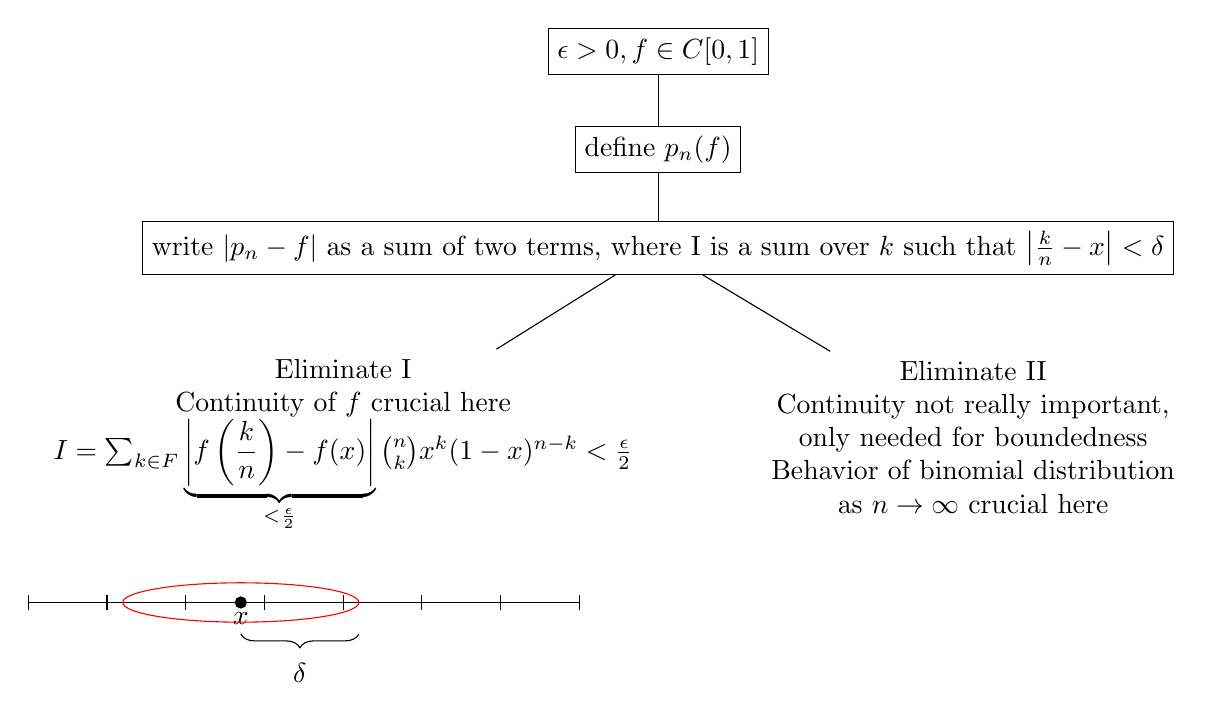
\begin{tikzpicture}[every text node part/.style={align=center}]
    \node (a) [draw] at (0, 0) {$\epsilon > 0, f \in C[0, 1]$};
    \node (b) [draw] at (0, -1.25) {define $p_n(f)$};
    \node (c) [draw] at (0, -2.5) {write $|p_n - f|$ as a sum of two terms, where I is a sum over $k$ such that $\left|\frac{k}{n} - x\right| < \delta$};
    \node (d) at (-4, -5) {Eliminate I \\ Continuity of $f$ crucial here \\ $I = \sum_{k \in F}\underbrace{\left|f\left(\frac{k}{n}\right) - f(x)\right|}_{< \frac{\epsilon}{2}} \binom{n}{k} x^k (1 - x)^{n - k} < \frac{\epsilon}{2}$};
    \node (e) at (4, -4.9) {Eliminate II \\ Continuity not really important, \\ only needed for boundedness \\ Behavior of binomial distribution \\ as $n \to \infty$ crucial here};
    \draw (a) -- (b) -- (c);
    \draw (c) -- (d);
    \draw (c) -- (e);
    \draw (-8, -7) -- (-1, -7);
    \foreach \x in {-8, -7, ..., -1}
    \draw[black] (\x, -7.1) -- (\x, -6.9);
    \draw[fill=black] (-5.3, -7) circle (2pt) node[below] {$x$};
    \draw[red] (-5.3, -7) ellipse (1.5 and 0.25);
    \draw[decorate, decoration={brace, amplitude=5pt}] (-3.8, -7.4) -- (-5.3, -7.4) node[black, midway, yshift=-0.5cm] {$\delta$};
  \end{tikzpicture}
\end{figure}

\noindent {\bf Question:} How do binomial probabilities $\binom{n}{k} x^k (1 - x)^k$ behave as $n \to \infty$?

\noindent {\bf Answer:} They sum to $1$, but their weight $\xrightarrow{n \to \infty} 0$ away from $x$.

\begin{figure}[H]
  \centering
  \begin{subfigure}{0.49\textwidth}
    \centering
    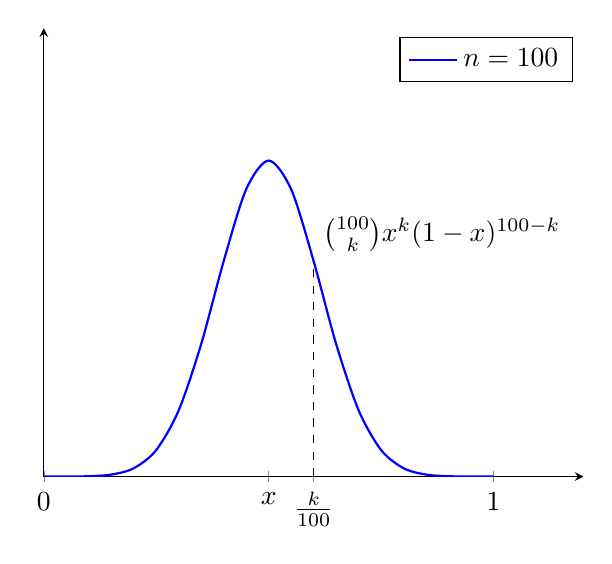
\begin{tikzpicture}[
        declare function={binom(\x,\n,\p)=\n!/(\x!*(\n-\x)!)*\p^\x*(1-\p)^(\n-\x);}
      ]
      \begin{axis}[
          xmin=0,
          xmax=1.2,
          ymin=0,
          ymax=0.25,
          xtick={0, 0.5, 0.6, 1},
          xticklabels={$0$, $x$, $\frac{k}{100}$, $1$},
          ymajorticks=false,
          axis x line=bottom,
          axis y line=left,
        ]
        \addplot[thick, blue, samples at={0,1,...,20}, smooth](x/20,{binom(x, 20, 0.5)});
        \draw[dashed] (axis cs:0.6, 0) -- (axis cs:0.6, 0.12013) node[above right] {$\binom{100}{k} x^k (1 - x)^{100 - k}$};
        \addlegendentry{$n = 100$}
      \end{axis}
    \end{tikzpicture}
  \end{subfigure}
  \begin{subfigure}{0.49\textwidth}
    \centering
    \begin{tikzpicture}[
        declare function={binom(\x,\n,\p)=\n!/(\x!*(\n-\x)!)*\p^\x*(1-\p)^(\n-\x);}
      ]
      \begin{axis}[
          xmin=0,
          xmax=1.2,
          ymin=0,
          ymax=0.25,
          xtick={0, 0.5, 0.6, 1},
          xticklabels={$0$, $x$, $\frac{k}{1000}$, $1$},
          ymajorticks=false,
          axis x line=bottom,
          axis y line=left,
        ]
        \addplot[thick, blue, samples at={0,1,...,100}, smooth](x/100,{binom(x, 100, 0.5)});
        \draw[dashed] (axis cs:0.6, 0) -- (axis cs:0.6, 0.01084) node[above right, xshift=-0.25cm, yshift=0.5cm] {$\binom{1000}{k} x^k (1 - x)^{1000 - k}$};
        \addlegendentry{$n = 1000$}
      \end{axis}
    \end{tikzpicture}
  \end{subfigure}
\end{figure}

All the mass of binomial probabilities eventually {\bf concentrates} near $x$:
$$ p_n(x) = \sum_{k = 0}^n f\left(\frac{k}{n}\right) \binom{n}{k} x^k (1 - x)^{n - k}. $$
$\frac{B(n, x)}{n}$ converges weakly to the {\bf Dirac delta} at $x$ as $n \to \infty$.

\begin{remark}
  \normalfont Suppose $f \in C(\RR) \text{ or } C(X)$, for an arbitrary metric space $X$. Polynomials $p(x) = a_0 + a_1 x + \ldots + a_n x^n \to \pm \infty$ as $n \to \infty$, so uniform convergence is not possible in general.
\end{remark}

\end{document}
